\documentclass[../defence.tex]{subfiles}

\begin{document}


  \begin{frame}{Alumina membranes - corrugations}
    \begin{columns}[onlytextwidth, T]
      \column{\dimexpr\linewidth / 2}
        \scalebox{0.6}{
          \tikzsetnextfilename{cp_iso}
          \begin{tikzpicture}
              \def\PrelMin{.86}
              \def\PrelMax{1}
              \def\TransMin{1e-8}
              \def\TransMax{10}
              \def\LfMin{0}
              \def\LfMax{1}
              %
              \begin{axis}[
                /tikz/line join=bevel,
                %width=0.8*\textwidth,
                %height=0.5*\textwidth,
                grid,
                %axis y line*=left,
                legend style={at={(0,1)}, legend columns=1, anchor=north west},
                every axis plot,
                line width = 1pt,
                %	minor x tick num= ,
                %	minor y tick num= ,
                xmin = \PrelMin, xmax = \PrelMax,
                ymin = \LfMin, ymax = \LfMax,
                xlabel = {Relative pressure $P_\mathrm{rel}$},
                ylabel = {Liquid fraction $LF$},
                ytick = {0,0.25,0.50,0.75,1},
                title=Closed pores,
                ]
                % Add plots
                \addplot[mark=none, color=red] table [x=Prel,y=liquid_fraction]{tikz/graphs/296_op_cp_comparison/296b_cp_cond_1.txt};
                \addlegendentry{$LF_\mathrm{cond}^\mathrm{296b}$}
                \addplot[mark=none, color=blue] table [x=Prel,y=liquid_fraction]{tikz/graphs/296_op_cp_comparison/296b_cp_evap_1.txt};
                \addlegendentry{$LF_\mathrm{evap}^\mathrm{296b}$}
              \end{axis}
          \end{tikzpicture}}
        \pause

      \column{\dimexpr\linewidth / 2}
        \begin{block}{Corrugations}
          The appearance of the hysteresis is assumed to be due to \textbf{intra pore corrugations}.
        \end{block}
        \scalebox{0.6}{
          \tikzsetnextfilename{corrugations}
          %\tikzexternaldisable
          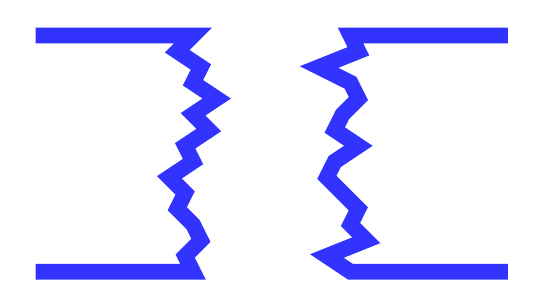
\begin{tikzpicture}
            \draw[color=blue!80, line width=2mm] (0,0)--(2,0)--(1.9,0.2)--(2.1,0.4)--(2,0.6)--(1.8,0.8)--(1.9,1)--(1.7,1.2)--(2,1.4)--(1.9,1.6)--(2.2,1.8)--(2,2)--(2.3,2.2)--(2,2.4)--(2.1,2.6)--(1.8,2.8)--(2,3)--(0,3);
              \draw[color=blue!80, line width=2mm] (6,0)--(4,0)--(3.7,0.2)--(4.2,0.4)--(4,0.6)--(4.1,0.8)--(3.9,1)--(3.7,1.2)--(3.8,1.4)--(4.1,1.6)--(3.8,1.8)--(3.9,2)--(4.1,2.2)--(4,2.4)--(3.6,2.6)--(4.1,2.8)--(4,3)--(6,3);
          \end{tikzpicture}}
    \end{columns}
  \end{frame}

\end{document}
